\documentclass[11pt,a4paper]{article}
\title{TFW: Preliminary results for class 150 train}
\usepackage{cite}
\usepackage{hyperref}
\usepackage{textcomp}
\usepackage{amssymb}
\usepackage{subcaption}
\usepackage{amsfonts}
\newcommand{\norm}[1]{\left\lVert#1\right\rVert}
\usepackage[left=2cm,right=2cm,top=2cm,bottom=3cm]{geometry}
\usepackage{amsmath}
\setlength\parindent{0pt}
\usepackage{float}
\usepackage{placeins}
\pretolerance=10000
\tolerance=2000
\emergencystretch=10pt
\author{Lucy Henley, Joshua Moore, Timothy Ostler \& Thomas Woolley\footnote{moorej16@cardiff.ac.uk, henleyl1@cardiff.ac.uk, ostlert@cardiff.ac.uk,woolleyt1@cardiff.ac.uk}}
\usepackage{graphicx}
\graphicspath{{./matlab_and_plots/}}
\begin{document}
\maketitle

\section*{Key points}
\begin{itemize}
\item We have run our seat selection code over the class 150 train
\item We achieved a maximum seat occupancy, with a $2$m social distancing measure, of approximately $22\%$
\item We have developed a web-based application for the class 150 train seating, available \href{https://lucyhenley.shinyapps.io/TFW_socialdistancing/}{here}.
\end{itemize}

\section*{What we could do next}
\begin{itemize}
\item Add other classes of train to the app
\item Include passenger direction to the analysis; a 1m social distance may be sufficient for passengers facing away from each other
\end{itemize}



\section*{Methods and results}
Following our discussions, we added the seating arrangements for the class 150 train to our app. Distance calculations are taken from the centre point of each seat. The results of the seat selection algorithm are displayed in Figure \ref{Demonstration_pics} and in Table \ref{tab:performance}.


\begin{figure*}[ht!]
\centering
\begin{subfigure}[h]{0.95\linewidth}
\centering
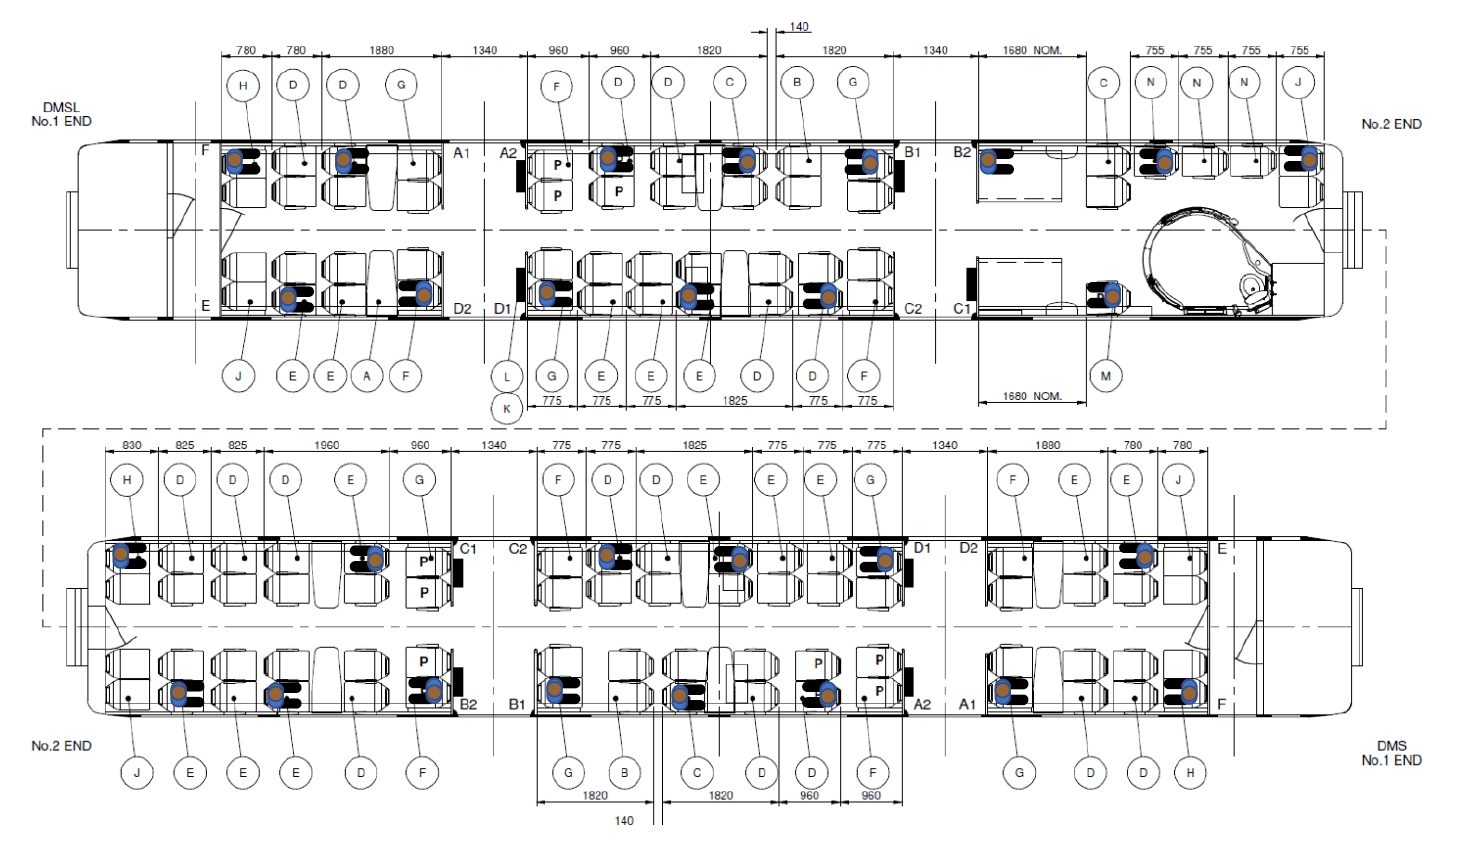
\includegraphics[scale = 0.6]{floorplan150.png}
\caption{The seating arrangement for the class 150 train.}
\label{Reference}
\end{subfigure}
~
\begin{subfigure}[h]{0.49\linewidth}
\centering
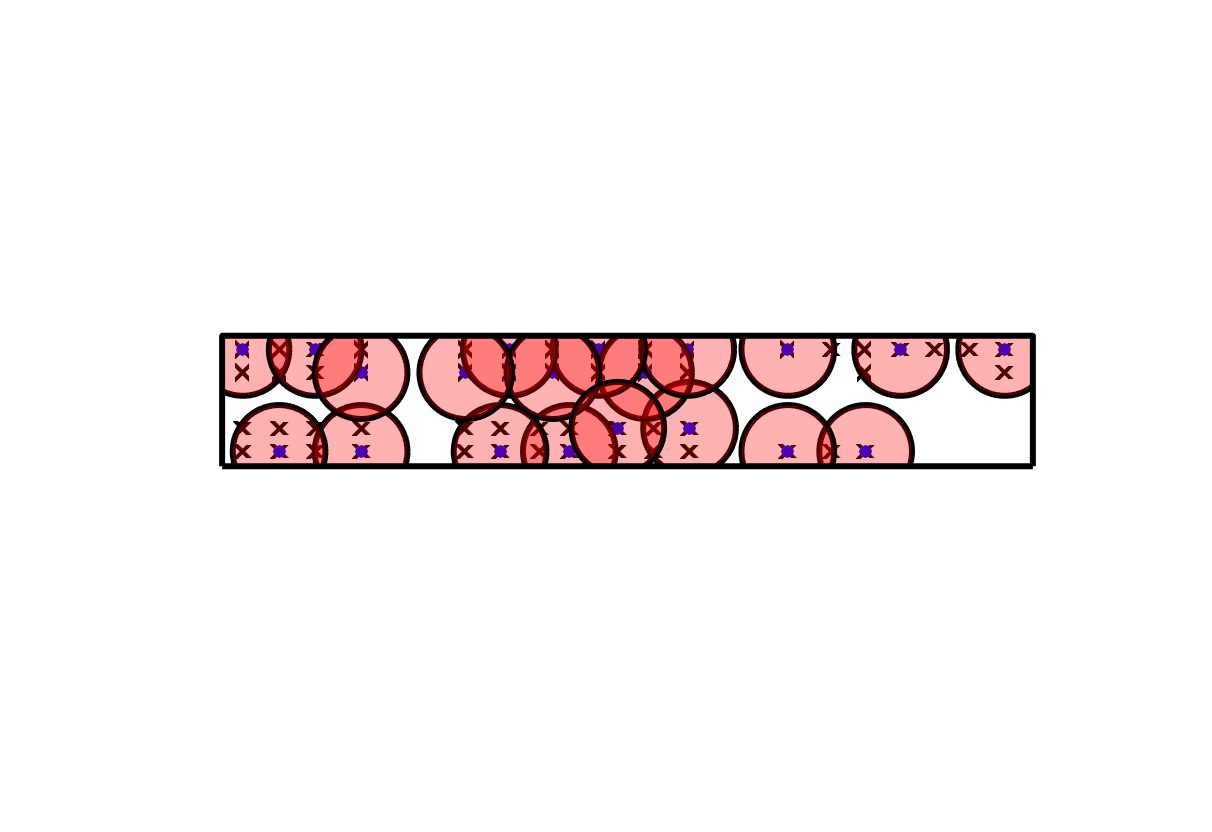
\includegraphics[width = \linewidth]{class150_first_car_1m.png}
\caption{A sample layout for carriage 1 with a social distancing measure of $1$ metres. $20$ seats are available.}
\label{OneMetre1}
\end{subfigure}
~
\begin{subfigure}[h]{0.490\linewidth}
\centering
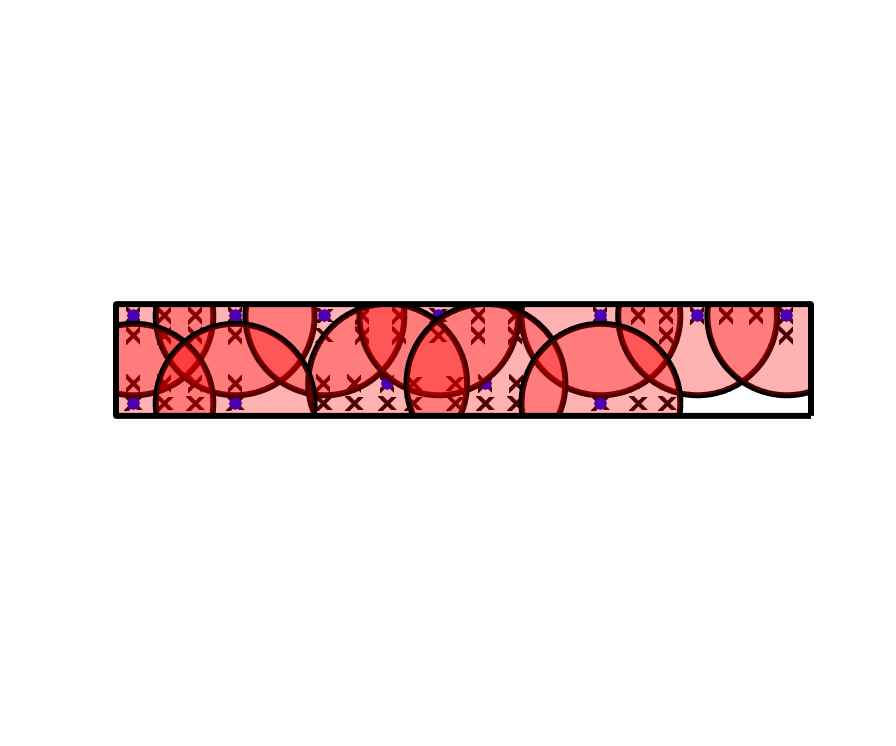
\includegraphics[width = \linewidth]{class150_first_car_2m.png}
\caption{A sample layout for carriage 1 with a social distancing measure of $2$ metres. $13$ seats are available.}
\label{TwoMetre1}
\end{subfigure}
~
\begin{subfigure}[h]{0.49\linewidth}
\centering
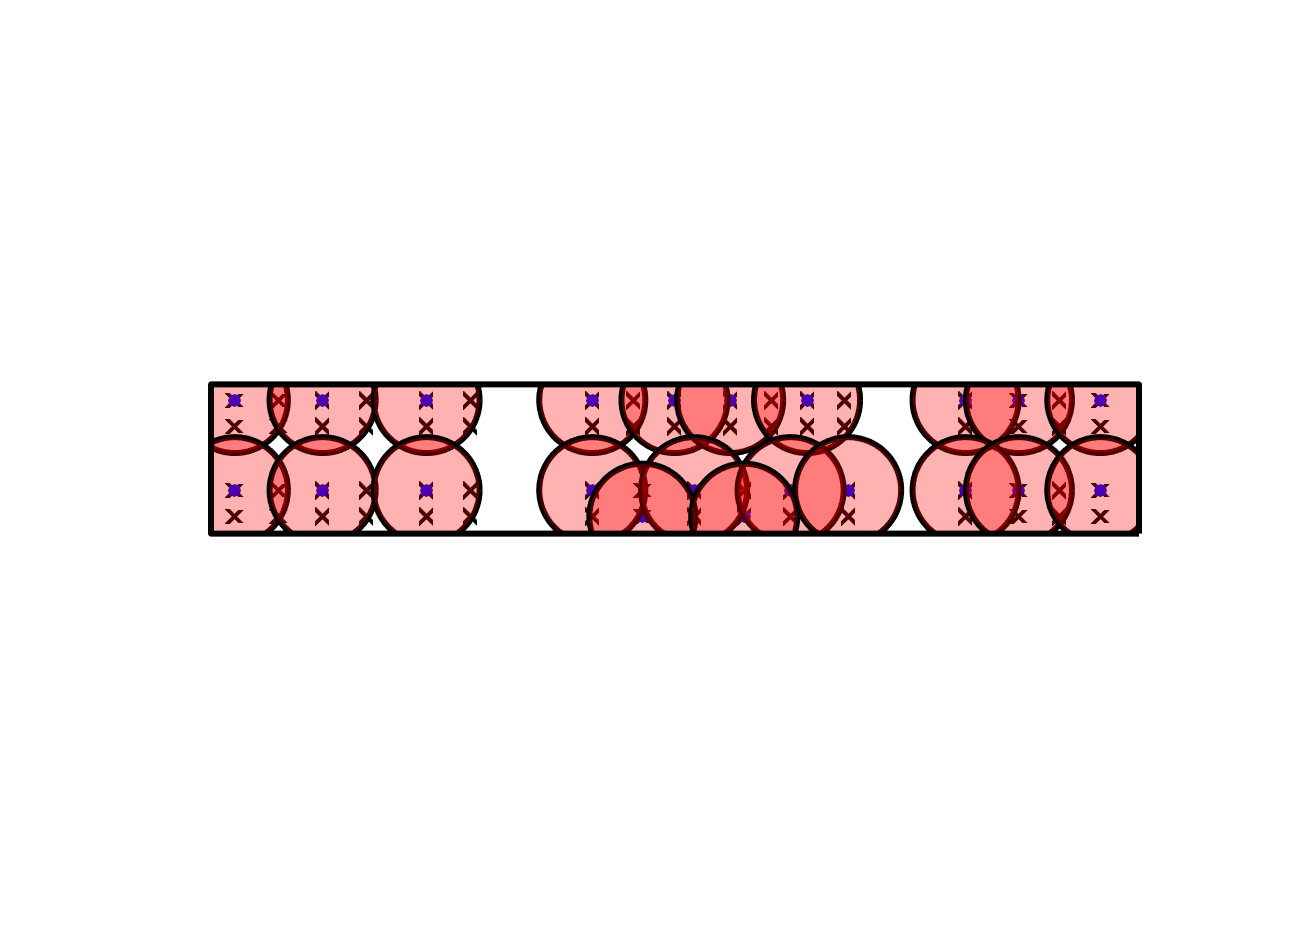
\includegraphics[width = \linewidth]{class150_second_car_1m.png}
\caption{A sample layout for carriage 2 with a social distancing measure of $1$ metres. $22$ seats are available.}
\label{OneMetre2}
\end{subfigure}
~
\begin{subfigure}[h]{0.490\linewidth}
\centering
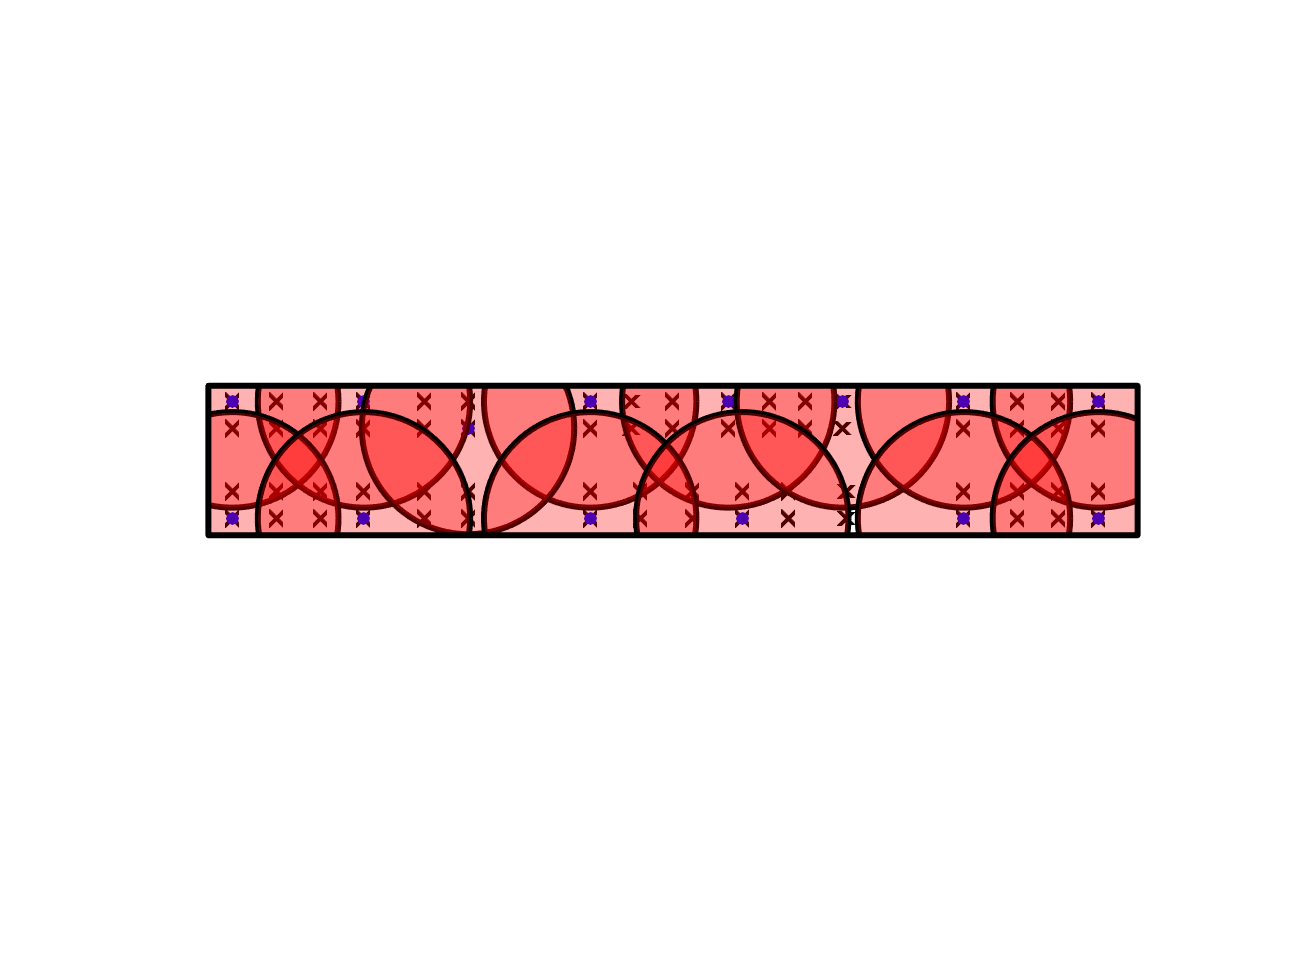
\includegraphics[width = \linewidth]{class150_second_car_2m.png}
\caption{A sample layout for carriage 2 with a social distancing measure of $2$ metres. $14$ seats are available.}
\label{TwoMetre2}
\end{subfigure}
\caption{A proposed seating layout given by the app for $1$ and $2$ metre social distancing for both carriages of the class 150 train. Seat locations are marked with crosses, available seats are marked with dots and the `region of safety' is denoted by a circle around the available seats. Overlapping circles imply that certain regions are exposed to contamination from multiple sources, but no available seats are located in these regions. }
\label{Demonstration_pics}
\end{figure*}


\begin{table}[ht!]
\begin{center}
 \begin{tabular}{|c |c|}
 \hline
& \textbf{Maximum capacity at $2$m social distancing }\\
 \hline
 Benchmark &   28 (23\%)\\
 \hline
 Cardiff App  & 27 (22\%)\\
\hline
\end{tabular}
\end{center}
\caption{Comparison of the performance of the Cardiff seat finding app against the benchmark provided in the supplied report.}
\label{tab:performance}
\end{table}


As demonstrated in Table \ref{tab:performance}, we can very quickly achieve similar occupancy rates in the train without violating social distancing measures. Given more time, we can develop methods for taking passenger direction into account, allowing for higher occupancy rates.

\section*{Prospective developments for improving optimality}
Our app always provides seating arrangements that obey social distancing measures, and provides locally optimal solutions which are similar the given benchmarks. Returning the  absolute optimum arrangement, however, is a lot more difficult because the problem is what is known as `NP-hard'.  Simply put, the only way to guarantee you have the most possible seats used is to try every possible order of seat checking, and pick the one which has the most seats used. Actually trying out every seat ordering would take a very long time; there are more ways to order $120$ seats than there are particles in the universe.\\

What we can do, though, is develop techniques to check our solutions and continuously improve upon them where possible. At a cost of additional time and computing power to implement, these methods would improve the likelihood we have found the best possible seating arrangement, allowing us to potentially further improve on our already powerful result.\\

\end{document}
